\noindent\textbf{Multi-armed bandits (MAB).} We consider a basic multi-armed bandit variant, \emph{stochastic Bernoulli bandits}. There are $K$ possible actions (\emph{arms}), indexed as $[K]:=\{1,\ldots,K\}$. Each arm $a$ is associated with mean reward $\mu_a\in[0,1]$, which is unknown.
An agent interacts with the environment for $T$ time steps, where in each time step $t\in [T]$ the agent selects an arm $a_t \in [K]$ and receives a reward $r_t\in\{0,1\}$ drawn independently from a Bernoulli distribution with mean $\mu_{a_t}$. Thus, the MAB instance is determined by the mean rewards $\rbr{\mu_a:\,a\in[K]}$ and the time horizon $T$. The goal is to maximize the total reward, which roughly corresponds to identifying the \emph{best arm}: an arm with the highest mean reward.
A key feature of the MAB setup is that rewards for arms not chosen by the agent are not revealed, so exploration is necessary to identify the best arm.


We focus on MAB instances where the best arm has mean reward $\mu^\star = 0.5+\Delta/2$ for a parameter $\Delta>0$, while all other arms have mean reward $\mu = 0.5-\Delta/2$ (so, $\Delta = \mu^\star-\mu$ is the \emph{gap} between the best and the second-best arm).
The main instance we consider has $K=5$ arms and gap $\Delta=0.2$. We call this the \hard instance, as we also consider an \easy instance with $K=4$ and $\Delta=0.5$.%
\footnote{A larger gap $\Delta$ makes it easier to distinguish arms, while smaller $K$ means there are fewer alternatives to explore.}


\xhdr{Prompts.}
We employ LLMs to operate as decision making agents that interact with MAB instances by prompting them
with a description of the MAB problem (including the time horizon $T$) and the history of interaction thus far. Our prompt design allows several independent choices.
First is a ``scenario'', which provides a grounding for the decision making problem, positioning the LLM either a) as an agent choosing \emph{buttons} to press, or b) as a recommendation engine displaying \emph{advertisements} to users.
Second, we specify a ``framing'' as either a) explicitly \emph{suggestive} of the need to balance exploration and exploitation, or b) \emph{neutral}.
Third, the history can be presented as a) a \emph{raw} list over rounds, or it can b) be \emph{summarized} via number of plays and average rewards of each arm.
Fourth, the requested final answer can be a) a single \emph{arm}, or b) a \emph{distribution} over arms. 
Finally, we either a) request the answer only, or b) also allow the LLM to provide a ``chain-of-thought" (CoT) explanation.
Altogether, these choices lead to $2^5=32$ prompt designs, illustrated in~\pref{fig:prompts}.
More details about the prompt design, including examples, are provided in~\pref{app:prompts}.


The most basic prompt design from the options above uses the buttons scenario, neutral framing, and raw history, and requests the LLM to return only an arm with no CoT.
Each of the five possible modifications to this prompt can potentially help the LLM, and our experiments evaluate this.
For example, both the advertising scenario and suggestive framing might help invoke the LLM's knowledge of bandit algorithms (as bandit algorithms are commonly used in content recommendation).
History summarization might help if the LLM cannot reliably summarize history itself (perhaps due to arithmetic errors%
\footnote{\Eg LLMs sometimes fail at basic arithmetic \citep{gao2023pal,liu2024exposing}, though this is likely to improve in the near future via better training and/or integrating calculator-like tools.})
and/or does not fully realize that it should. Returning a distribution might help if the LLM can identify a good distribution, but fails to correctly sample from it. Finally, chain-of-thought is known to help in a wide variety of LLM scenarios \citep{wei2022chain,malach2023auto}, even when used in a zero-shot manner~\citep{kojima2022large} as we do here.

\begin{wrapfigure}{r}{0.5\textwidth}
  \vspace{-8mm}
  \begin{center}
    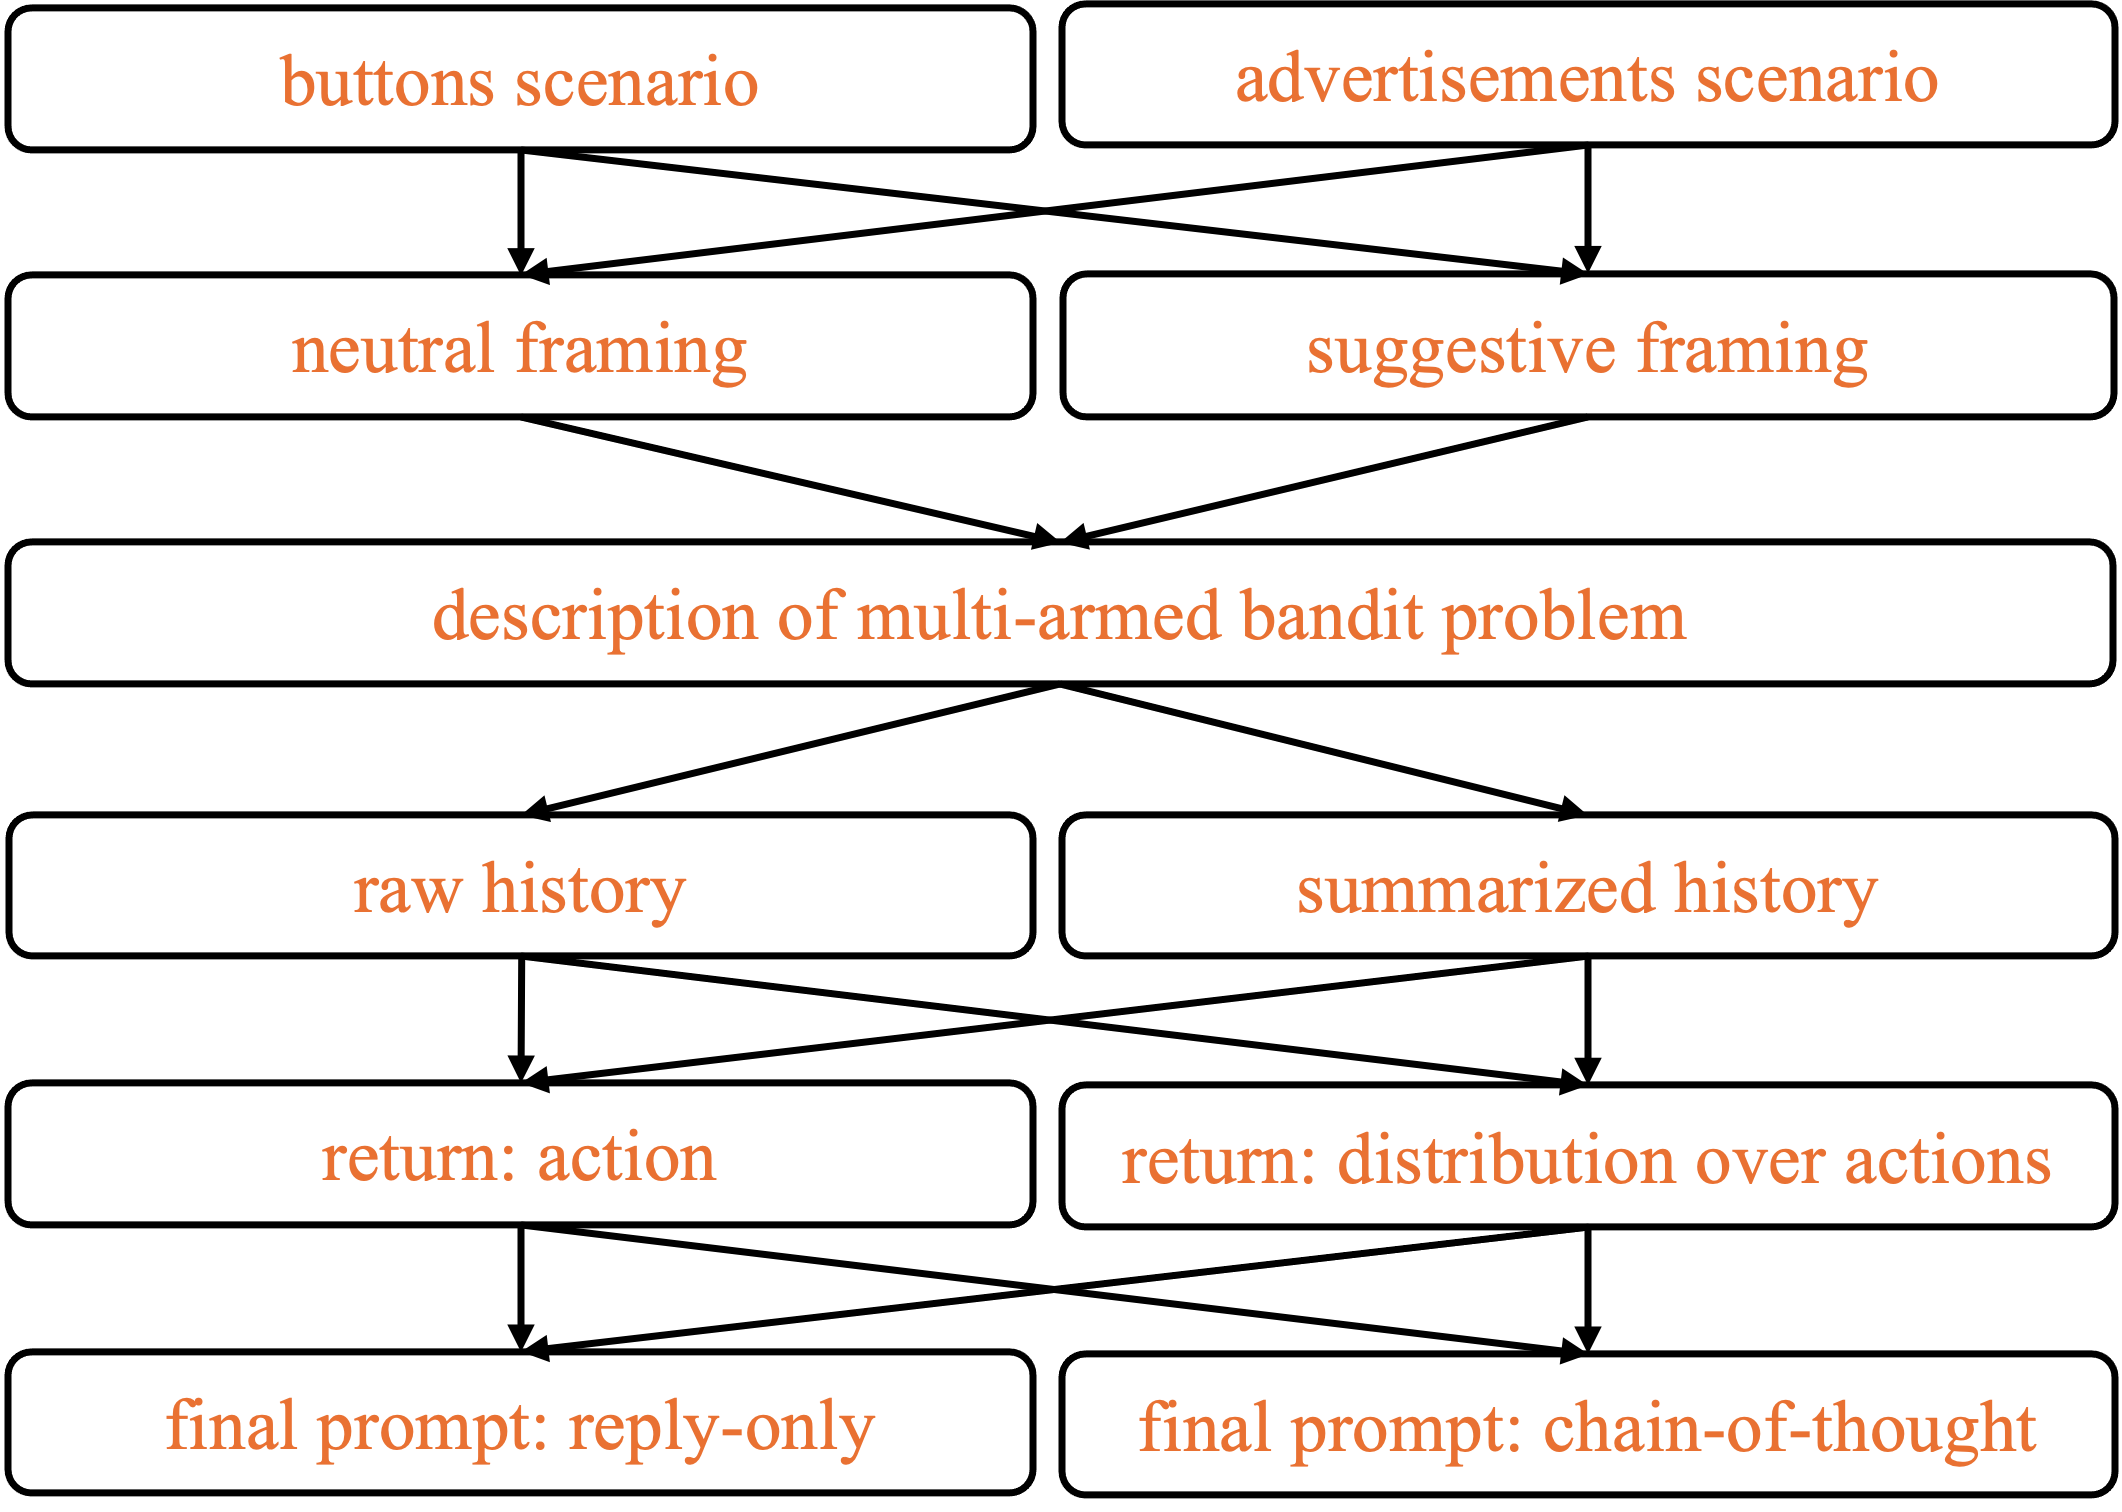
\includegraphics[width=0.5\textwidth]{./prompt-Jan28.png}
  \end{center}
  \vspace{-0.7cm}
  \caption{Prompt designs; see Figure~\ref{fig:prompts-text} for a more detailed view. A prompt is generated by traversing the graph from top to bottom.}
  \vspace{-2mm}
  \label{fig:prompts}
\end{wrapfigure}

Prompts are presented to each LLM using both system and user messages (exposed by all three LLM APIs). %
The system message presents information about the scenario and framing and prompts the LLM about whether to use CoT and whether (and how) to return a distribution.
The user message presents the history and reminds the LLM about how to format its response.
For \gptfour only, we found that prompting the LLM to use CoT in the system prompt did not reliably elicit CoT outputs, so---for \gptfour only---we also consider a \emph{reinforced CoT} prompt design that additionally reminds the LLM to use CoT at the end of the user prompt.
See~\pref{app:prompts} for examples.




\xhdr{LLM configurations.}
We experiment with three LLMs: \gptthree, \gptfour, and \llama.\footnote{Specifically: \textsc{GPT-3.5-Turbo-0613} (released 06/13/2023), \textsc{GPT-4-0613} (released 06/13/2023), and \textsc{Llama2-13B-chat} quantized to 4-bits~\citep{dettmers2023case}.}
In addition to the prompt variations above, we also consider two choices for the temperature parameter, $0$ and $1$.
A temperature of $0$ forces the LLM to be deterministic and therefore isolates the ``deliberate'' exploration behavior of the LLM itself.
A temperature of $1$ provides a source of external randomness in the LLM responses, which may or may not result in randomization among the arms.
Allowing the LLM to return a distribution instead of a single arm 
also provides external randomness (as we sample from the returned distribution); to
isolate sources of randomness, we do not consider temperature $1$ with ``return distribution" prompt designs.\loose

We refer to the tuple (prompt design, temperature) as the \emph{LLM configuration}. We identify each configuration with a 5-letter ``code" $L_1 L_2 L_3 L_4 L_5$, with letters $L_i$ denoting the choices:
\begin{itemize}
\setlength{\itemsep}{0pt}
\item $L_1$: `B' or `A' for, resp., buttons or advertisements scenario;
\item $L_2$: `N' or `S' for, resp., neutral or suggestive framing;
\item $L_3$: `R' or `S' for, resp., raw or summarized history;
\item$L_4$: `C' or `$\widetilde{\text{C}}$' or `N' for, resp., chain-of-thought, reinforced CoT, or no CoT.
\item $L_5$: '0', '1' or 'D' for, resp., temperature and returning a distribution (with temperature $0$).
\end{itemize}
We refer to ``BNRN0" as the \emph{basic} configuration going forward.
Most of our experiments consider the ``buttons'' scenario, and we use the ``advertisements'' scenario primarily as a robustness check.

For \gptthree and \llama, we do not consider reinforced CoT as it is not required to reliably elicit CoT outputs; thus, we have 48 configurations total for these two LLMs.
For \gptfour, we primarily used reinforced CoT, but did experiment with some standard CoT prompt designs; thus, there are 72 configurations total for \gptfour.

\paragraph{Baselines}
For baselines, we consider two standard MAB algorithms, \ucb \citep{bandits-ucb1} and Thompson Sampling (\ts) \citep{Thompson-1933}, which are optimal in a certain theoretical sense and also reasonably effective in practice. We also consider the \greedy algorithm, which does not explore and is known to fail.%
\footnote{\label{fn:greedy}In each round, \greedy chooses an arm with the largest average reward so far. The algorithm is initialized with one sample of each arm. It \emph{fails} in that with constant probability, it never chooses the best arm after initialization.}
While all three baselines have tunable parameters,
we perform no parameter tuning (see~\pref{sec:bg} for a detailed description of each algorithm with parameter settings). In addition to these baselines, some of our experiments include the the \EpsGreedy algorithm\footnote{\label{fn:eps-greedy}\EpsGreedy is a standard MAB algorithm which in each round chooses an arm uniformly at random with a given probability $\eps$, and exploits (\ie mimics \greedy) otherwise.} with various choices of $\eps$ to quantitatively demonstrate tradeoffs between exploration and exploitation.
We ran $1000$ replicates for each baseline and each MAB instance (with rewards realized independently across the replicates).


\xhdr{Scale of the experiments.}
Our main set of experiments has time horizon $T=100$.
To account for randomness in rewards (and possibly in the LLM, via temperature) we ran $N \in \{10, 20\}$ replicates for each LLM configuration and each bandit instance, with rewards generated independently across the replicates.
As a robustness check, we ran a single experiment on \gptfour with the basic configuration for $T=500$ rounds (with $N=20$), and obtained consistent/stronger conclusions, depicted in \pref{fig:long}(a).

In more detail, for \gptthree we used $N=20$ replicates across all $48$ prompt configurations, resulting in $\approx 200K$ queries in total.
\gptfour was an order of magnitude more expensive, considerably slower on throughput, and subject to unpredictable throttling.
As such, we only used $N=10$ replicates across $10$ representative prompt configurations.\footnote{Precisely, $N=10$ for the buttons scenario, and $N=3$ for the robustness check with the advertisements scenario.}
For additional robustness checks, we ran four \gptfour configurations with $T=200$, two for $N=20$ replicates and two for $N=40$ replicates.
In total, this resulted in ${\approx}50K$ queries issued to \gptfour.
\llama was essentially free from our perspective (since it was locally hosted), but its performance was consistently sub-par; we limited our experiments to the \hard MAB instance, $32$ configurations, and $N=10$ replicates.



We emphasize that bandit experiments with LLMs are quite costly in terms of money and time. They take $N \cdot T$ LLM queries for each LLM configuration and each MAB instance being tested.
Both $N$ and $T$ must be relatively large to obtain statistically meaningful results:
$N$ governs the significance level and must be large to overcome randomness in reward realizations, while $T$ governs the effect size and must be large so that good algorithms have enough time to identify the optimal arm.
Both issues are more pronounced in harder MAB instances (many arms $K$ and/or small gap $\Delta$), but exploration failures also tend to be less frequent in (very) easy MAB instances.%
\footnote{For example, \greedy always succeeds when the gap is $\Delta=1$, \ie there is no noise, and trivially succeeds with probability at least $(1+\Delta)^2/4$ when the initial samples evaluate to $1$ for the good arm and $0$ for the bad arm.}
Further, we need to cover the space of possible prompt designs, which is essentially infinitely large, to ensure that our findings do not overfit to one particular design.
Thus, ideally we would take $N$, $T$, the number of MAB instances, and the number of prompts to be rather large, but doing so is not practically feasible.%
\footnote{Raw-history prompts and chain-of-thought outputs are particularly expensive, as LLM APIs bill per token.}
Instead, we use
moderately small gap $\Delta=0.2$, moderately large choices for $N \in \{10,20\}$ and $T=100$, and the prompt design space as described above.


As we will see below, these choices (specifically, $N \in \{10,20\}$
and $T=100$ and $\Delta=0.2$) do not provide enough statistical power
to distinguish between successful and unsuccessful methods based
solely on accumulated rewards. In lieu of further increasing the scale
of the experiments, which is not practically feasible, we rely
on \emph{surrogate statistics} which can be detected at our moderate
scale, and which are highly suggestive of long-term/persistent
exploration failures. Our robustness checks with larger $T$ and $N$, as well as qualitative findings that we report below provide supporting evidence for this methodology.








